\documentclass[skript.tex]{subfiles}

\begin{document}
	\begin{bem}
		Die Dimension einer Mannigfaltigkeit ist wohldefiniert. ---
		Eine nichtleere Teilmenge des $\R^n$ ist genau dann eine
		$n$-dimensionale Mannigfaltigkeit, wenn sie offen ist.
	\end{bem}
	
	\begin{notat}[Lineare Algebra]
		Sei $X$ ein endlich-dimensionaler (reeller) Vektorraum mit innerem Produkt $\skp{\bcdot}{\bcdot}$.
		Das \emph{orthogonale Komplement} $V^\perp$ eines Unterraums $V \sbs X$
		ist durch
		\[
			V^\perp = \{ x\in X \mid \skp{x}{v}=0 \quad \forall v\in V\}
		\]
		gegeben, und wir haben $V \oplus V^\perp=X$.
		Ist $Y$ ein weiterer endlich-dimensionaler Vektorraum
		und $A \colon X \to Y$ eine lineare Abbildung, so setzen wir
		\begin{alignat*}{2}
			\kernel A &= \{x\in X \mid Ax=0\} &&\sbs X, \\
			\image A &= \{Ax \mid x\in X\} &&\sbs Y,
		\end{alignat*}
		und es gilt $\underbrace{\dim\kernel}_{\text{Defekt}} A + \underbrace{\dim\image}_{\text{Rang}} A = \dim X$.
	\end{notat}

	\begin{theorem}
		Für $m,n\in\N$, $m\le n$ und eine nichtleere Menge $M \sbs \R^n$
		sind die folgenden Aussagen äquivalent:
		\begin{enumerate}[(i)]
			\item \emph{(Untermannigfaltigkeit)}\quad
			Für jedes $\xi \in M$ gibt es eine offene Umgebung $\Omega  \sbs \R^n$
			von $\xi$, eine Menge $U \sbs\R^{m}$ und eine Immersion $ \phi\in C^1(U,\R^n)$,
			die $U$ homöomorph auf
			\[
				M\cap\Omega =  \phi(U)
			\]
			abbildet.
			
			\item \begin{minipage}[t]{.55\textwidth}
				\emph{(Gleichungsdefinierte Mannigfaltigkeit)}\quad
				Zu jedem ${\xi \in M}$ gibt es eine offene Umgebung $\Omega \sbs \R^n$ von $\xi$ und eine Abbildung $f \in C^1(\Omega,\R^{n-m})$ mit
				$ \rank D f(x)=n-m \:\forall x\in\Omega$ und
				\[
					M \cap \Omega = f^{-1}(\{0_{\R^{n-m}}\}).
				\]
			\end{minipage}
			\hfill
			\begin{minipage}[t][.2\textwidth][b]{.3\textwidth}
				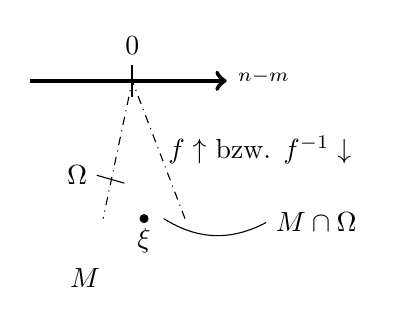
\begin{tikzpicture}
					\saucer{0}{0}{.75};
					\draw[->,ultra thick] (.5,2.5)--(3,2.5) node[right]{$\R^{n-m}$};
					\draw[thick] (1.8,2.3)--(1.8,2.7) node[above]{$0$};
					\draw[dashdotted] (2.47,.75)-- node[right]{$f\uparrow$ bzw. $f^{-1}\downarrow$ } (1.8,2.5)--(1.43,.75);
					
					\node at (1.2,0){$M$};
					\filldraw (1.95,.75) circle[radius=.05] node[below]{$\xi$};
					\draw (1.7,1.2)--(1.35,1.3) node[left]{$\Omega$};
					\draw (3.5,.7) node[right]{$M\cap\Omega$} to[bend left] (2.2,.75);
				\end{tikzpicture}
			\end{minipage}
			
			\item \emph{(Graphendarstellung)}\quad
			Zu jedem $\xi \in M$ gibt es eine offene Umgebung $\Omega \sbs \R^n$ von $\xi$,
			eine offene Menge $U \sbs\R^{m}$ und ein $g \in C^1(U,\R^{n-m})$ mit
			\[
				M\cap\Omega = \Pi(\graph g),
			\]
			wobei $\Pi \in \mathrm{GL}(n)$ eine Permutationsmatrix ist.
		\end{enumerate}
	\end{theorem}
	Eine Permutationsmatrix $\Pi$ ist durch einen Zykel\footnote{zyklische Permutation, siehe Lineare Algebra I} $\sigma\in\mf{S}_{n}$
	eindeutig charakterisiert, und es gilt
	$\Pi e_{j}=e_{\sigma(j)}$ für $j=1,\dotsc, n$.
	\begin{proof}
		\emph{„(i)$\implies$(ii)“}:\quad Wir konstruieren eine Funktion $f$ mithilfe des Umkehrsatzes.\\
		Sei also $M$ eine $m$-dimensionale Untermannigfaltigkeit des $\R^n$ wie in \emph{(i)} und \\
		$\eta = \phi^{-1}(\xi) \in U$. Da $\phi$ eine Immersion ist, besitzt $D \phi(\eta)$ einen vollen Rang und die Spalten von $D\phi$ spannen einen linearen Unterraum $T$ auf.
		\begin{center}
			\fbox{
				\begin{minipage}{.4\textwidth}
					\vspace{.4\textwidth}
					Grafik folgt in Kürze.
					\vspace{.4\textwidth}
				\end{minipage}
			}
		\end{center}
		Mit $P_T$ bezeichnen wir die orthogonale Projektion $\R^n \to T\sbs\R^n$. Weiterhin setzen wir $\phi_T \ceq P_T \circ \phi \colon U \to T \sbs \R^n$. Insbesondere gilt $\rank D\phi_T = m$, denn
		\[
			D\phi_T = D(P_T \circ \phi) =\footnotemark \underbrace{((D P_T)\circ\phi)}_{= P_T} D\phi.
		\]
		\footnotetext{
			$A = P_T, v\in\R^n$
			\[
				\frac{A(x+\tau v)-A(x)}{\tau} = Av \implies D A = A
			\]
		}
		Entsprechend ist
		\[
			D\phi_T(\R^n) = P_T\underbrace{D\phi(\R^n)}_{= T}=T.
		\]
		Nach einem Koordinatenwechsel können wir $T=\R^m\times\{0_{\R^{n-m}}\}$ annehmen und setzen außerdem $N = \{0_{\R^{n}}\}\times\R^{n-m}$ und $\phi_N = P_N \circ \phi \colon U \to N$, wobei $P_N$ die orthogonale Projektion auf $N$ bezeichnet.\\
		Der Umkehrsatz liefert nun eine offene Umgebung $\wt{U} \sbs U$ von $\eta$, so dass
		\[
			\phi_T|_{\wt{U}} \colon \wt{U} \to \phi_T(\wt{U}) \eqqcolon \wt{V}
		\]
		ein Diffeomorphismus ist.\\
		Insbesondere gibt es eine inverse Abbildung
		\[
			\psi \coloneqq (\phi_T|_{\wt{U}})^{-1} \in C^1(\wt{V},\wt{U}).
		\]
		Wir wählen $\wt{\Omega} \sbs \Omega$ mit $\xi \in \Omega$ und $\phi^{-1}(\wt{\Omega} \cap M) \sbs \wt{U}$. Weiter setzen wir $\Omega^\ast=(\wt{V} \oplus N)\cap\wt{\Omega} \sbs \Omega$, d.\,h. für jedes $x\in\Omega^\ast$ gibt es eine Zerlegung $x=x_T+x_N$ wobei $x_T \in \wt{V} \sbs T$ und $x_N \in N$.\\
		Mit
		\[
			f(x) = f(x_T+x_N) = \underbrace{x_N}_{\in N}-\underbrace{\phi_N(\psi(x_T))}_{\in N}
		\]
		erhalten wir eine Abbildung $f \in C^1(\Omega^\ast,N)$.\\
		Aus $D_N f = \mathds{1}_{n-m}$ erhalten wir $\rank D\psi(x) = \dim N = n-m \quad\forall x \in \Omega^\ast$.\\
		Somit bleibt $\Omega^\ast \cap M = \{x\in\Omega^\ast \mid f(x) = 0\}$ zu zeigen.\\
		Sei hierzu $x \in \Omega^\ast$, d.\,h. $x \in \wt{\Omega}$ mit $x = x_T+x_N,\ x_T\in\wt{V}\sbs T,\ x_N \in N$.\\
		Nun setzen wir $u=\psi(x_T)\in\wt{U}$, also $x_T = \phi_T(u)$.\\
		Wir haben $f(x)=0 \iff x_N = \phi_N(u) \iff x = \phi(u) \in M \cap \Omega$.\\
		
		\emph{„(ii)$\implies$(iii)“}:\quad Sei $M$ eine gleichungsdefinierte Mannigfaltigkeit. Zu $x \in M$ wählen wir $\Omega$ und $f$ aus \emph{(ii)}. Nach Umnummerierung der Koordinaten (was auf die Permuationsmatrix $\Pi$ führt) erhalten wir $D_z f(\xi)\in\mathrm{GL}(n-m)$, wobei $x=(y,z)\in\R^m\times\R^{n-m}$.\\
		Aus dem Satz über implizite Funktionen gewinnen wir eine offene Umgebung\\$U \times V \sbs \R^m\times\R^{n-m}$ von $\xi = (\eta,\zeta)$ und eine Funktion $g \in C^1(U,V)$ mit
		\[
			\graph g = \{(y,z) \in U \times V \mid f(y,z) = 0\} = M \cap (U \times V).
		\]
		
		\emph{(iii)$\implies$(i)}:\quad Unter den Voraussetzungen von \emph{iii} erhalten wir mit
		\[
			\phi \colon y \mapsto \Pi(y,g(y))
		\]
		eine Abbildung aus $C^1(U,\R^n)$. Folglich ist $\phi(U)=M\cap\Omega$ und es bleibt zu zeigen, dass $\phi$ eine Immersion ist und einen Homöomorphismus liefert.\\
		Aus der Definition liest man unmittelbar die Injektivität von $\phi$ sowie $\rank D\phi=m$ ab.\\Nach Voraussetzung ist $\phi$ stetig und die Stetigkeit von $\phi^{-1}$ sieht man wie folgt:
		
		Eine konvergente Folge in $\image\phi$ lässt sich durch eine Folge $(y_k)_{k\in\N}\sbs U$ mit\\
		$\phi(y_k) = \Pi(y_k,g(y_k))\to w\in\image\phi\sbs\R^n$
		darstellen.\\
		Mit $(y,z)=\Pi^{-1}(w)$
		ergibt sich $(y_k,g(y_k)) \to (y,z)$ und insbesondere $y_k\to y$.\\
		Somit ist $M$ eine Mannigfaltigkeit.
	\end{proof}
	
	\begin{defin}[Tangentialraum/Normalraum]
		Sei $M \sbs \R^n$ eine $m$-dimensionale Mannigfaltigkeit und $\xi \in M$. Ein Vektor $v \in \R^n$ heißt \emph{Tangentialvektor an $M$ im Punkt $\xi$}, falls es eine Kurve $\gamma \in C^1((-\epsilon,\epsilon),M),\ \epsilon>0$, mit $\gamma(0)=\xi,\ \gamma'(0) = v$ gibt.\\
		Die Menge aller Tangentialvektoren wird \emph{Tangentialraum an $M$ im Punkt $\xi \in M$} genannt und mit $T_\xi M$ bezeichnet.\\
		Der \emph{Normalraum an $M$ in $\xi$} ist das orthogonale Komplement $N_\xi M = (T_\xi M)^\perp$.
	\end{defin}

	\begin{theorem}
		Sei $M\sbs\Rn$ eine $m$-dimensionale Mannigfaltigkeit, $\xi \in M$, $m \leq n$.\\
		Sei $\phi \in C^1(U,\Rn)$ eine lokale Parametrisierung von $M$ an $\xi$ und sei $f$ wie in \emph{Satz 9\,(iii)}.\\
		Dann gilt
		\begin{alignat*}{2}
			T_\xi M &= \image D\phi(0) &&=\kernel Df(\xi),\\
			N_\xi M &= (\image D\phi(0))^\perp &&=\spann(\nabla f_1(\xi),\dotsc,\nabla f_{n-m}(\xi)).
		\end{alignat*}
		Insbesondere ist $T_\xi M$ wirklich ein Vektorraum und wir haben
		\[
			\dim T_\xi M = m, \qquad \dim N_\xi M = n-m.
		\]
	\end{theorem}
	\begin{proof}
		Wir können \OE\ $\phi(0) = \xi$ annehmen.\\
		Wir zeigen zunächst $\image D\phi(0) \sbs T_\xi M$.\\
		Für $w\in\image D\phi(0)$ gibt es ein
		$u\in\R^m$ mit $w=D\phi(0)u$.\\
		Für $\gamma(t)=\phi(tu)$ gilt $\gamma(0) = \phi(0) = \xi$ und $\gamma'(0) = D\phi(0)u=w$.\\
		Damit ist $w \in T_\xi M$.\\
		Weiterhin ist $T_\xi M \sbs \kernel Df(\xi)$.\\
		Sei hierzu $v \in T_\xi M$. Definitionsgemäß gibt es eine
		Kurve $\gamma \colon (-\epsilon,\epsilon) \to M$ mit $\gamma(0)=\xi$ und $\gamma'(0)=v$. Wir können $\epsilon>0$ so klein wählen, dass $\image\gamma$ in $M\cap\Omega$ enthalten ist, wobei $\Omega$ die
		in \emph{Satz 9\,(ii)} angegebene offene Menge bezeichnet.\\
		Wegen $\image\gamma \sbs M$ gilt insbesondere
		$f\circ\gamma\equiv0$, also
		\[
			0 = (f\circ\gamma)'(0) = Df(\gamma(0))\gamma'(0) = Df(\xi)v,
		\]
		folglich ist $v \in \kernel Df(\xi)$. Damit haben wir insgesamt:
		\[
			\image D\phi(0) \sbs T_\xi M \sbs \kernel Df(\xi)
		\]
		Wegen $\dim\image D\phi(0) = \rank D\phi(0) = m$ und
		\[
			\dim\kernel Df(\xi) = n - \rank Df(\xi) = n-(n-m) = m
		\]
		folgt die behauptete Identität.\\
		Insbesondere ist $T_\xi M$ ein $m$-dimensionaler Vektorraum.\\
		Wir erhalten nach Definition $N_\xi M = (T_\xi M)^\perp
		= (\image D\phi(0))^\perp$.\\
		Sei nun $w = \nabla f_j(\xi)$ für ein $j=1,\dotsc,n-m$ und $v \in T_\xi M$.\\
		Wir erhalten
		\[
			\skp{w}{v} = \mathlarger\sum_{k=1}^n \ddel{f_j}{x_k}(\xi) v_k = (Df(\xi)v)_j = 0,
		\]
		da $T_\xi M = \kernel Df(\xi)$.\\
		Nun folgt $w \perp T_\xi M$, also $w \in N_\xi M$, und mithin
		\[
			\spann(\nabla f_1(\xi),\dotsc,\nabla f_{n-m}(\xi)) \sbs N_\xi M.
		\]
		Wegen $\rank Df(\xi) = n-m$ handelt es sich bei beiden Mengen um Vektorräume der Dimension $n-m$ und diese sind folglich gleich.
	\end{proof}

	\begin{theorem}[Tangentialebene]
		Für jeden Punkt $\xi$ einer Mannigfaltigkeit $M$ ist mit $\Xi = \xi + T_\xi M$
		\[
			\frac{1}{r} \sup\{\dist(x,\Xi) \mid x\in M\cap B_{r}(\xi)\} \xrightarrow{r \searrow 0} 0.
		\]
	\end{theorem}
	\begin{center}
		\fbox{
			\begin{minipage}{.4\textwidth}
				\vspace{.4\textwidth}
				Grafik folgt in Kürze.
				\vspace{.4\textwidth}
			\end{minipage}
		}
	\end{center}
\end{document}